In jeder Anwendung gibt es Teile bzw. Module, die aus allen Komponenten des Programms erreichbar sein sollen
(z.B. Logger Controller oder Datum Controller), und es gibt auch Klassen, die regelmäßig instanziert werden.

Das Problem dabei ist, dass in das neue erstellte Objekt die Utility Controllers immer neben den anderen Argumenten 
mitübergeben werden müssen. Das erschwert die Lesbarkeit des Codes und kann eine Reihe an Änderungen an vielen Stellen mit sich ziehen,
falls man die Konstruktoren ändert.

Es gibt folgende Möglichkeiten das Problem zu lösen:
\begin{itemize}
    \item Globale Objekte bzw. Instanzen (z.B. OOP Design Pattern \textbf{Singleton} \ref{kap:gof:singleton})
    \item Initialisiereung von den Entsprechenden Instanzen und Übergeben in dem Konstruktor (OOP Sprachen)
    oder mittels einer Settermethode.
\end{itemize}

Bei der ersten Implementierung hat man das Problem, dass die benutzten Utility Controllers nicht ersetzbar sind.
D.h. man kann dann alle Module sehr schwer mit Unittests abdecken, denn es werden immer auch die Utility Controllers mitgetestet.
Ein weiteres Problem besteht darin, dass alle Utility Controllers eine Infrastruktur benutzen.
(z.B. Logs in dem Datenbank speichern). Jeder Test wird dadurch deutlich länger laufen.
Da es auch reele Infrastruktur sein wird, wird es die Parallelisierung des Tests deutlich erschwert, denn 
der Zustand der benutzten Infrastruktur durch mehrere unabhängig voneinander laufendenen Tests geändert wird.

Bei der zweiten Möglichkeit müssen alle Utility Controllers entweder bei der Initialisiereung im Konstruktor 
der jeweiligen Instanzen übergeben oder mittels einer Settermethode der Instanz.
Die erste Möglichkeit führt zu einer längeren Parameterliste, die die Lesbarkeit des Codes erschwert.
Die zweite Möglichkeitführt dazu, dass der Aufruf der Methode von dem Softwareentwickler vergessen werden kann.

Das Problem lässt sich zum Beispiel durch OOP design pattern \textbf{Factory} (Kapitel \ref{kap:gof:factory}), das die Utility Controllers bereits
enthält und bei der Initialisierung entsprechend in die Konstruktor übergibt. 
Jeder Teil des Programms besitzt eine Referenz auf der Instanz der Fabrik, 
die ein kürzeres (kleinere Übergabeparameterliste) Interface für das Erstellen von verschieden Instanzen anbietet.
Alle Module bzw. Klassen lassen sich somit auch mit Unittests
abdecken, da die Utility Controllers entsprechend gemockt werden können. 

In der Abbildung \ref{fig:CDControllerWithUtility} ist die Verbindung jedes \textbf{Controller}s mit den Utility Controllers als Klassendiagramm dargestellt.
    
\begin{figure}[H]
    \centering
    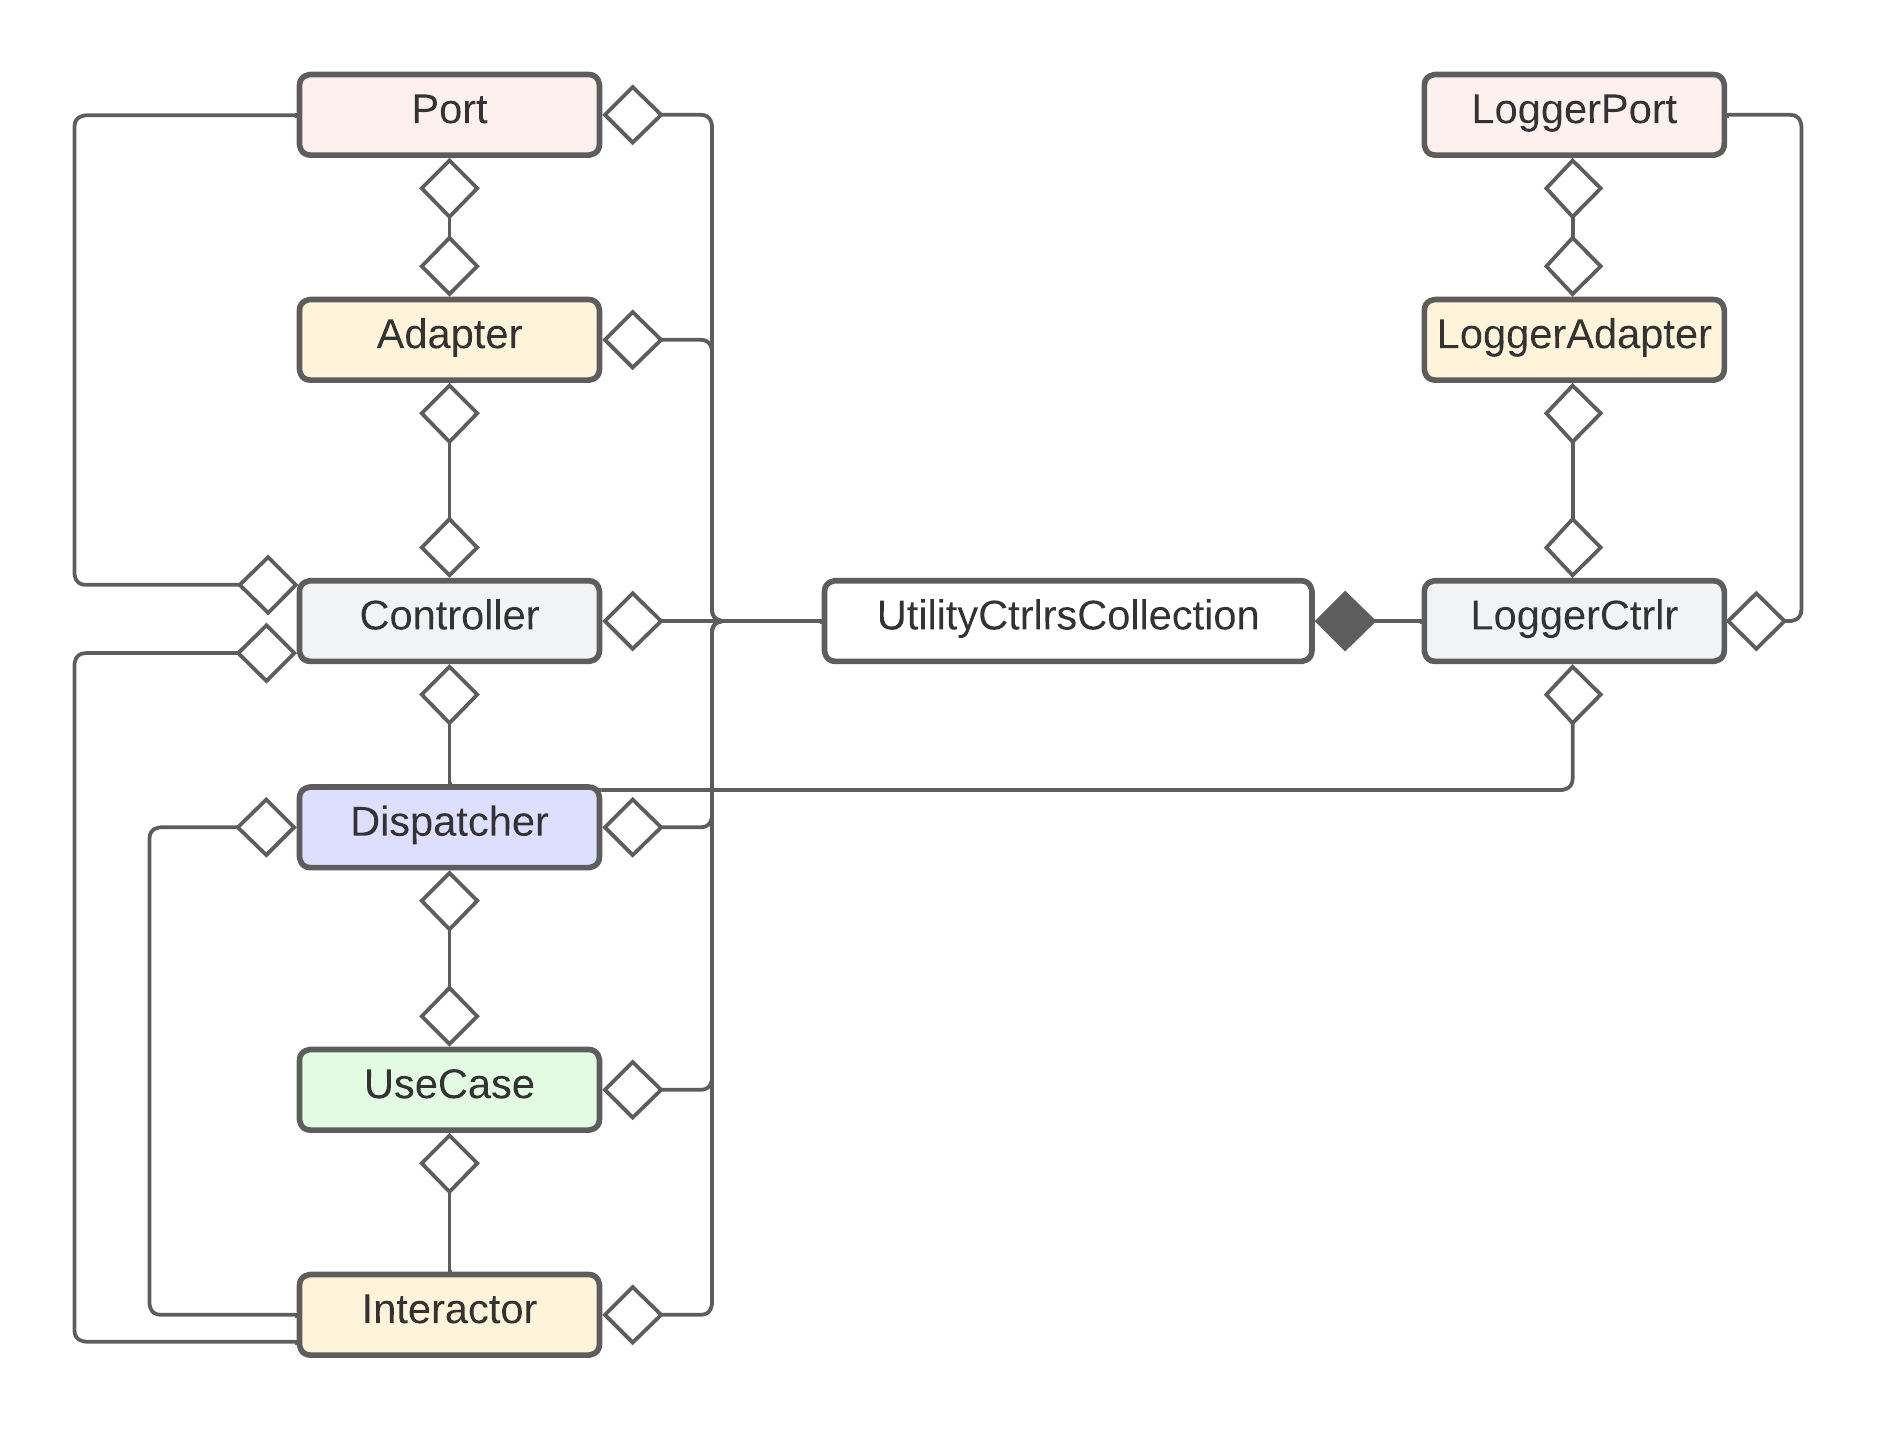
\includegraphics[width=12cm]{./images/KlassendiagramMitUtilityControllers.png}
     \caption[Objektendiagramm mit Utility Controllers]{Objektendiagramm mit Utility Controllers \footnotemark}
     \label{fig:CDControllerWithUtility}
\end{figure}
